%!TEX TS-program = xelatex
% Исходная версия шаблона --- 
% https://www.writelatex.com/coursera/latex/5.1
\documentclass[c, dvipsnames]{beamer}  % [t], [c], или [b] --- вертикальное 
%\documentclass[handout, dvipsnames, c]{beamer} % Раздаточный материал (на слайдах всё сразу)
%выравнивание на слайдах (верх, центр, низ)
%\documentclass[handout, dvipsnames]{beamer} % Раздаточный материал (на слайдах всё сразу)
%\documentclass[aspectratio=169, dvipsnames]{beamer} % Соотношение сторон
\setbeamertemplate{navigation symbols}{}%remove navigation symbols

%\usetheme{Berkeley} % Тема оформленияLLL
%\usetheme{Bergen}
%\usetheme{CambridgeUS}
\usetheme{Boadilla}

\usecolortheme{crane} % Цветовая схема

%\useoutertheme{infolines} % Навигация 
%\useoutertheme{tree}
%\useoutertheme{miniframes}
%\useoutertheme{shadow}
%\useoutertheme{sidebar}
%\useoutertheme{smoothbars}
%\useoutertheme{smoothtree}
%\useoutertheme{split}
%\useoutertheme{default}


%\useinnertheme{circles}
\useinnertheme{rectangles}
%\useinnertheme{rounded}
%\useinnertheme{inmargin}


%%% Работа с русским языком
\usepackage[english,russian]{babel}   %% загружает пакет многоязыковой вёрстки
\usepackage{fontspec}      %% подготавливает загрузку шрифтов Open Type, True Type и др.
\defaultfontfeatures{Ligatures={TeX},Renderer=Basic}  %% свойства шрифтов по умолчанию
\setmainfont[Ligatures={TeX,Historic}]{Arial} %% задаёт основной шрифт документа
\setsansfont{Arial}                    %% задаёт шрифт без засечек
\setmonofont{Arial}
\usepackage{indentfirst}
\frenchspacing



%% Beamer по-русски
\newtheorem{rtheorem}{Теорема}
\newtheorem{rproof}{Доказательство}
\newtheorem{rexample}{Пример}

%%% Дополнительная работа с математикой
\usepackage{amsmath,amsfonts,amssymb,amsthm,mathtools} % AMS
\usepackage{icomma} % "Умная" запятая: $0,2$ --- число, $0, 2$ --- перечисление

%% Номера формул
\mathtoolsset{showonlyrefs=true} % Показывать номера только у тех формул, на которые есть \eqref{} в тексте.
%\usepackage{leqno} % Нумерация формул слева

%% Свои команды
\DeclareMathOperator{\sgn}{\mathop{sgn}}

%% Перенос знаков в формулах (по Львовскому)
\newcommand*{\hm}[1]{#1\nobreak\discretionary{}
{\hbox{$\mathsurround=0pt #1$}}{}}

%%% Работа с картинками
\usepackage{graphicx}  % Для вставки рисунков
\graphicspath{{images/}{images2/}}  % папки с картинками
\setlength\fboxsep{3pt} % Отступ рамки \fbox{} от рисунка
\setlength\fboxrule{1pt} % Толщина линий рамки \fbox{}
\usepackage{wrapfig} % Обтекание рисунков текстом

%%% Работа с таблицами
\usepackage{array,tabularx,tabulary,booktabs} % Дополнительная работа с таблицами
\usepackage{longtable}  % Длинные таблицы
\usepackage{multirow} % Слияние строк в таблице

%%% Программирование
\usepackage{etoolbox} % логические операторы

%%% Другие пакеты
\usepackage{lastpage} % Узнать, сколько всего страниц в документе.
%\usepackage{soul} % Модификаторы начертания
\usepackage{csquotes} % Еще инструменты для ссылок
\usepackage{multicol} % Несколько колонок


\usepackage{hyperref}
\usepackage{xcolor}
\hypersetup{        % Гиперссылки
    unicode=true,           % русские буквы в раздела PDF
    pdftitle={Заголовок},   % Заголовок
    pdfauthor={Автор},      % Автор
    pdfsubject={Тема},      % Тема
    pdfcreator={Создатель}, % Создатель
    pdfproducer={Производитель}, % Производитель
    pdfkeywords={keyword1} {key2} {key3}, % Ключевые слова
    colorlinks=true,        % false: ссылки в рамках; true: цветные ссылки
    linkcolor=,          % внутренние ссылки
    citecolor=green,        % на библиографию
    filecolor=magenta,      % на файлы
    urlcolor=blue           % на URL
} 

\usepackage{dcolumn}

%fffff3
\definecolor{backgr}{RGB}{146,26,29}
\definecolor{backgr1}{RGB}{230,43,37}
\definecolor{ex1}{RGB}{231,142,36}
\definecolor{ex2}{RGB}{249,155,28}
\definecolor{ex3}{RGB}{242,103,36}

\definecolor{red}{RGB}{230,43,37}
%\setbeamercolor{normal text}{fg=black,bg=backgr}
\setbeamercolor{frametitle}{bg=backgr,fg=white}
%\setbeamercolor{footline}{bg=backgr,fg=white}
%\setbeamercolor{normal text}{bg=yellow}
%\setbeamercolor{section in toc}{fg=yellow}
%\setbeamercolor{subsection in toc}{fg=blue}

% How to change colour of Navigation Bar in Beamer -  много интересного

%Пример команд, задающих внешний вид блока
\setbeamercolor{block title}{fg=white,bg=ex1}
\setbeamerfont{block title}{family=\sffamily}
\setbeamercolor{block body}{bg=white}
\setbeamertemplate{blocks}[rounded][shadow=fasle]
\setbeamercolor{title}{bg=backgr, fg=white}
\setbeamercolor{alerted text}{fg=backgr1}

\newlength\subtitwd
\setlength\subtitwd{4cm}% change the width here

\makeatletter
\newcommand\titlegraphicii[1]{\def\inserttitlegraphicii{#1}}
\titlegraphicii{}



%\newcommand\superviser[1]{\def\insertsuperviser{Научный руководитель: #1}}
\newcommand\superviser[1]{\def\insertsuperviser{  #1}}



\superviser{}

\setbeamertemplate{title page}
{
  \vbox{}
   {\usebeamercolor[fg]{titlegraphic} \hspace{0.35ex} \inserttitlegraphic\hfill\inserttitlegraphicii \hspace{1ex} \par }\vspace{1.5ex}
  \begin{centering}
    \begin{beamercolorbox}[sep=8pt,center]{institute}
      \usebeamerfont{institute}\insertinstitute
    \end{beamercolorbox}
    \begin{beamercolorbox}[sep=8pt,center]{title}
    
      \usebeamerfont{title}\inserttitle\par%
      \ifx  \insertsubtitle\@empty%
      \else%
        \vskip0.5em%
        {\usebeamerfont{subtitle}\usebeamercolor[fg]{subtitle}\insertsubtitle\par}%
      \fi%     
    \end{beamercolorbox}%
    \vskip1em\par
    \begin{beamercolorbox}[sep=5pt,center]{date}
      \usebeamerfont{date}\insertdate
    \end{beamercolorbox}%\vskip0.5em
    \begin{beamercolorbox}[sep=5pt,center]{author}
      \usebeamerfont{author}\insertauthor
    \end{beamercolorbox}
        \begin{beamercolorbox}[sep=4pt,center]{institute}
      \usebeamerfont{institute}\insertsuperviser
    \end{beamercolorbox}
  \end{centering}
  %\vfill
}
\makeatother

\setbeamercolor{item projected}{bg=ex3}
\setbeamertemplate{enumerate items}[default]

\setbeamercolor{palette primary}{bg=white}
\setbeamercolor{palette primary}{fg=black}
\setbeamercolor{palette secondary}{bg=white}
\setbeamercolor{palette secondary}{fg=black}
\setbeamercolor{palette tertiary}{bg=white}
\setbeamercolor{palette tertiary}{fg=black}

\setbeamercolor{itemize item}{fg=ex3}
\setbeamercolor{itemize subitem}{fg=ex2}
\setbeamercolor{itemize subsubitem}{fg=ex1}

\setbeamercolor{enumerate item}{fg=ex3}
\setbeamercolor{enumerate subitem}{bg=ex3}
\setbeamercolor{enumerate subsubitem}{bg=ex3}


\setbeamertemplate{itemize subitem}{$\Rightarrow$}
\setbeamertemplate{itemize item}{$\blacktriangleright$}



\usepackage{todo}
\newcolumntype{a}{>{\columncolor{red}}c}


\usefonttheme{professionalfonts}

\title[   Моделирование финансовых рисков     ]{Моделирование финансовых рисков    рынка электрической энергии в России }
%\subtitle{Защита выпускной квалификационной работы}


%Stochastic Factors Affecting Commodity Prices: the Case of Russia

 \usepackage{amsmath}

\author[Касьянова Ксения]{Касьянова Ксения \\ \smallskip \scriptsize  }

%\superviser{ Научный руководитель }

%\author[Имя автора]{Имя автора \\ \smallskip \scriptsize \href{mailto:author@ranepa.ru}{author@ranepa.ru} \\ \smallskip  \href{http://ranepa.ru}{http://ranepa.ru} }

\institute[РАНХиГС]{ \uppercase{
  Институт отраслевых рынков и инфраструктуры}}
\date{}



\titlegraphic{
\includegraphics[scale=0.5]{logo1}}
\titlegraphicii{
\includegraphics[scale=0.5]{logo2}}

\begin{document}

\frame[plain]{\titlepage}	% Титульный слайд

\section{Intro}

\begin{frame}[shrink=3]
\frametitle{Цели и задачи} 


\begin{block}{Актуальность:}
	\begin{itemize}
		
		\item необходимость верно оценивать рыночные риски возникает у производителей электричества, желающих хеджировать  риски (1 час - 1 день),    финансовых посредников  торгующих контрактами на электроэнергию (1 день - 1 месяц), инвесторов (1 месяц - 1 год).
%		;
%		\item при решении UCP (Unit commitment problem) в производстве электроэнергии. 
%				
		
%		\item   фьючерсы недавно торгуются, в России биржа электричества молодая, Россия необычная страна)))).  


	\end{itemize}
\end{block}


\begin{block}{Гипотеза:}
	\begin{itemize}
		
		\item стандартные модели оценки риска не подходят для российской рынка, риск недооценен, добавление дополнительных факторов позволит получить более точные оценки риска. 
	
		
		%		\item   фьючерсы недавно торгуются, в России биржа электричества молодая, Россия необычная страна)))).  
		
		
	\end{itemize}
\end{block}


\begin{block}{Цель:}
	\begin{itemize}
		
		
		\item  разработка модели оценки риска,  учитывающей  особенности российского рынка электроэнергетики. 
		
		
%		 обладает своими особенностями, то  их учет при моделировании риска будет способствовать  Сравнить риски на российской бирже
		

		%		\item  выявление факторов, позволяющих улучшить прогнозы агрегированного временного ряда. 
		
	\end{itemize}
	
\end{block}

%никакого прогнозирования, не коммодити

%остановиться только на электричестве  (есть цены за 3 года - плавающее окно)

%Оформление: Только на русском, без значков эмита)))))))))


%альтернативы электричеству:  про нефть не особо, все внутренние товарные биржи ненастоящие и нужны ФАС для оценки, если внешние - не понятно какие котировки брать, если общие, то не понятно, какое влияние оказывает на наш рынок, если русские - не понятно кто торгует, в чем смысл, кто виноват и что делать


\end{frame}

\begin{frame}[shrink=3]
\frametitle{Цели и задачи} 


\begin{block}{Задачи:}


	\begin{itemize}
		
		\item  сравнение классических моделей оценки риска (VaR) на российских данных (можно попробовать применить к американским/европейским);
		
		\item определение причин, по которым в какие-то моменты риски были завышены/занижены;  

%		цель посчитать VaR в класическом  варианте, сравнить с реальными рисками, сказать, что риск был недоценен, улучшить с помощью изменения распределения
				
		\item  выявление факторов влияющих на цены на электричество: факторы также могут быть случайными,  описываться различными моделями: gmb - цены на другие ресурсы, запасы ресурса, pois/extr - климатические факторы, катастрофы/аварии, новости, политические факторы и др.); 
		  
		
%		\item  выбор моделей наилучшим образом описывающих цены на каждый из товаров;

		\item  проверка коинтегрированности факторов с ценами;

		\item  добавление факторов в модели оценки риска (например, вместо нормального распределения в VaR моделях использовать скорректированное распределение, учитывающее эти факторы);
		%\item  сравнение прогнозов по рядам второго и третьего уровня. 
		\item  сравнение модели с базовыми: определить, удалось ли решить проблему с неправильными оценками риска. 		
		
		
	\end{itemize}
	
\end{block}
\end{frame}


\begin{frame}[shrink=5]
\frametitle{Специфика рынка электроэнергетики} 

\begin{itemize}
	\item невозможность хранения => проблема обязательства энергоустановки (unit commitment)
	\item проблема с ограничениями ЛЭП (проблема решается единым оператором), возможность перенапряжения сети (в таком случае локальные цены отличаются от общеустановленных по системе) 
	\item цены на электричество определяются на РСВ, т.е. отсутствует непрерывность торговли, решения на все сутки принимаются на основании одного и того же информационного множества
	\item невозможность перераспределить волатильность цен по производственной цепочке 
	\item  цены имеют три уровня циклических колебаний: ежедневная, недельная, годовая (с резкими всплесками в январе)
	\item причины энергетических кризисов: изменения налогообложения, рыночные манипуляции, устаревшая инфраструктура, провалы рынка, национализация, излишняя зарегулированность, перебои с поставками топлива, резкое изменение климата,  доставка электричества дешевле стоимости производства 
	  
\end{itemize}


\end{frame}


\begin{frame}[shrink=5]
\frametitle{Специфика российского рынка} 


АТС


\end{frame}



\section{Price}

\begin{frame}[shrink=5]
\frametitle{Базовая модель описывающая цену на электричество} 


Модель Мертона (Merton’s Jump-Diffusion Model)

\begin{itemize}
	\item эмпирическое распределение имеет тяжелые хвосты, что не согласуется со стандартной моделью Блэка-Шоулза
	\item  в модель добавляется отдельная компонента, отвечающая за скачкообразность процесса (логнормально распределенные скачки порожденные пуассоновским потоком)    
\end{itemize}

Пусть $S_t$ - цена в момент $t$.

Риск-нейтральный диффузионно-скачкообразный процесс (jump-diffusion process), описывающий изменение цены на электричество:

$$dS_t/S_t=(r−\lambda \bar{k})dt+\sigma dW_t+kdq_t.$$

где $\sigma$ - волатильность диффузионной компоненты. 

Скачки порожденны составным процессом Пуассона  $q_t$  с параметром  $\lambda$, где $k$  - размах случайного скачка, причем:

$$ln(1 +k)\sim N(\gamma,\delta^2)$$

где среднее - $\bar{k} = E(k)=e^{\gamma + \delta^2/2}-1$



\end{frame}





\begin{frame}[shrink=5]
\frametitle{Специфика рынка электроэнергетики} 

На равновесие на рынке  электричества влияет 

\begin{itemize}
	\item  погодные условия (причем при более точном прогнозировании погодных условий можно уменьшить ошибку прогноза цены на электричество)
	\item  уровень ежедневной деловой активности 
	\item  доля ВИЭ (в т.ч. зависимых от погодных условий) 
	\item  решения принимаемые  экономическими агентами (оптимизация)
\end{itemize}

\end{frame}



\begin{frame}[shrink=5]
\frametitle{Основные экономические модели ценообразования на рынке электричества} 


\begin{itemize}
		\item  моделирование с учетом фундаментальных факторов (физических/экономических)
	\item модели типа Курно (в результате - цены выше чем в действительности)
	\item моделирование совокупной функции предложения (необходимо решить систему дифференциальных уравнений, вычислительно затратно, не уделяется внимание резким всплескам) 
	\item  моделирование поведения групп агентов  (необходимо для выявления сложных зависимостей, применяется совместно с другими моделями, высокие риски моделирования, так как согласование с теоретической моделью  и эмпирическими наблюдениями сильно зависит от предпосылок и понимания настоящей структуры рынка)

\end{itemize}

\end{frame}




\begin{frame}[shrink=5]
\frametitle{Анализ предметной отрасли} 


	
	\begin{table} \small\centering\setlength{\extrarowheight}{0.25em}
		
		\begin{tabular}{   >{\centering\footnotesize}p{5.5em} 
				>{\centering\footnotesize}p{10em}
				>{\centering\footnotesize\arraybackslash}p{20em} }\hline
			
			
			
			Авторы, год & Название работы &  Результат \\\hline 
			
			
			L. YANG, S. HAMORI (2018) & \href{https://www.worldscientific.com/doi/abs/10.1142/S2010495218500100}{MODELING THE DYNAMICS OF INTERNATIONAL AGRICULTURAL COMMODITY PRICES:A COMPARISON OF GARCH AND SV MODELS}  &    Основываясь на ежемесячных данных, скачкообразные процессы и асимметричный эффект не влияют на цены на сельскохозяйственную продукцию. Оценивая VaR для этих сельскохозяйственных товаров, мы обнаруживаем, что резкий рост цен на сельскохозяйственную продукцию в 2008 году мог быть вызван частой перебалансировкой портфелей. \\
			
			  Mária Bohdalová, Michal Greguš (2015) & \href{https://www.researchgate.net/publication/283243124_ESTIMATING_VALUE-AT-RISK_BASED_ON_NON-NORMAL_DISTRIBUTIONS}{ESTIMATING VALUE-AT-RISK BASED ON NON-NORMAL DISTRIBUTIONS}  &    Моделирование VaR в предположении, что ежедневные изменения цен iid не с нормальным распределением или   автокоррелированны  с через  динамику факторов риска \\
			
			
			
			Rainer Göb (2011) & \href{https://onlinelibrary.wiley.com/doi/abs/10.1002/qre.1238}{Estimating value at risk and conditional value at risk for count variables}  &    Эмпирические аспекты оценки риска с биномиальным распределением и распределении Пуассона. Особое внимание уделяется интервальной оценке мер риска.  \\\hline
			
%			H. Mostafaei et al.  (2013) & 
%		\href{https://dergipark.org.tr/en/download/article-file/361215}{A Methodology for the Choice of the Best Fitting Continuous-Time Stochastic Models of Crude Oil Price: The Case of Russia }   & Выбор стохастического процесса наилучшим образом, описывающего цену на нефть \\
%			 A. Murat,  E. Tokat (2009) & \href{https://www.sciencedirect.com/science/article/pii/S0140988308001096?via\%3Dihub}{Forecasting oil price movements with crack spread futures}
%			   &   Коинтегрированность цен  на нефть и фьючерсов на крэк-спред => прогнозы VECM with crack spread futures лучше, чем у VECM with crude oil futures. 



			
		\end{tabular}
	\end{table}


\end{frame}





\begin{frame}[shrink=5]
\frametitle{Данные} 


Данные по ценам на электричество за каждый час, начиная с 1.08.2013 по двум ценовым зонам: 

\begin{itemize}
	\item Объем полного планового потребления, МВт.ч
	\item Индекс равновесных цен на покупку электроэнергии, руб./МВт.ч.
	\item Объем покупки по регулируемым договорам, МВт.ч
	\item  Объем покупки на РСВ, МВт.ч	
	\item Объем продажи в обеспечение РД, МВт.ч	
%	\item  Максимальный индекс равновесной цены, руб./МВт.ч	\item Минимальный индекс равновесной цены, руб./МВт.ч
%	
	
\end{itemize}

Источник: \href{https://www.atsenergo.ru/results/rsv}{АТС}




%SPIMEX:
%
%- URALS
%
%- Биржевые индексы цен нефтепродуктов: 92, 95, ДТ, СУГ.
%
%НТБ:
%
%- Зерновые
%
%http://www.ntb.moex.com/ru/archive/Zakupki2016

% Please add the following required packages to your document preamble:
% \usepackage{multirow}
%		
%\begin{table}[]
%	
%	\small\centering\setlength{\extrarowheight}{0.25em}
%	
%	\begin{tabular}{   >{\centering\footnotesize}p{8em} 
%			>{\centering\footnotesize}p{4em} 
%			>{\centering\footnotesize}p{4em} 
%			>{\centering\footnotesize}p{4em} 
%			>{\centering\footnotesize\arraybackslash}p{6em} }\hline
%
%		
%		
%\multirow{2}{*}{\begin{tabular}[c]{@{}c@{}}Агрегированный\\ ряд\end{tabular}} & \multicolumn{3}{c}{Ряды второго уровня} & \multirow{2}{*}{\begin{tabular}[c]{@{}c@{}}Число рядов \\ третьего уровня\end{tabular}} \\
%& по регионам & по типам & по кластерам &  \\\hline
%ВВП ЕС & 28 & 10 & 25 & 280 \\
%ВВП США & 50 & 21 & 25 & 1050 \\
%ЕП РФ & 80 & 4 & 25 & 320\\\hline
%
%	\end{tabular}
%\end{table}
%
%
%\begin{table}[]
%	
%	\small\centering\setlength{\extrarowheight}{0.25em}
%	
%	
%	
%	\begin{tabular}{   >{\centering\footnotesize}p{8em} 
%			>{\centering\footnotesize}p{5em} 
%			>{\centering\footnotesize}p{5em} 
%			>{\centering\footnotesize}p{4em} 
%			>{\centering\footnotesize\arraybackslash}p{4em} }\hline
%		
%		\multirow{2}{*}{\begin{tabular}[c]{@{}c@{}}Агрегированный\\ ряд\end{tabular}} & \multirow{2}{*}{Сезонность} & \multirow{2}{*}{\begin{tabular}[c]{@{}c@{}}Число\\ наблюдений\end{tabular}} & \multicolumn{2}{c}{Кросс-валидация} \\
%		&  &  & \begin{tabular}[c]{@{}c@{}}число\\ подвыборок\end{tabular} & \begin{tabular}[c]{@{}c@{}}ширина\\ окна\end{tabular} \\\hline
%		ВВП ЕС & 4 & 75 & 6 & 48 \\
%		ВВП США & 4 & 54 & 6 & 28 \\
%		ЕП РФ & 12 & 157 & 5 & 84\\\hline
%	\end{tabular}
%\end{table}
%


\end{frame}



\begin{frame}[shrink=5]
\frametitle{Данные} 





\begin{figure}
	\centering
	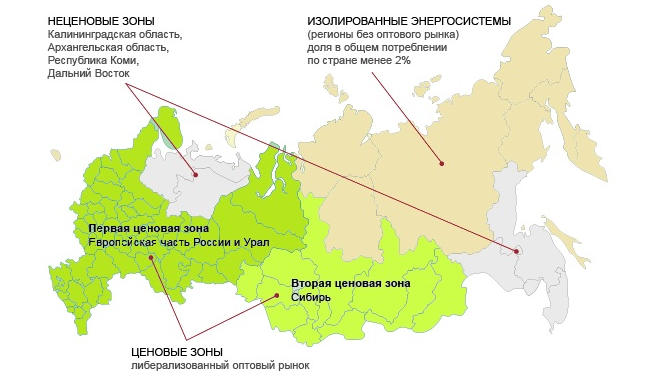
\includegraphics[width=0.7\linewidth]{screenshot003}
	\caption{ Ценовые зоны  }
	\label{fig:screenshot003}
\end{figure}

\end{frame}





\begin{frame}[shrink=5]
\frametitle{Данные} 





\begin{figure}
	\centering
	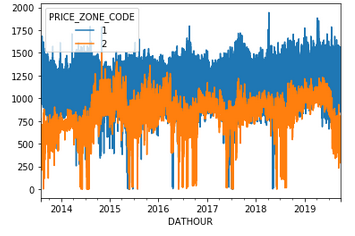
\includegraphics[width=0.7\linewidth]{screenshot002}
	\caption{ Почасовые цены в первой и второй ценовых зонах }
	\label{fig:screenshot002}
\end{figure}

\end{frame}

\begin{frame}[shrink=5]
\frametitle{Специфика российского рынка} 

Примеры:

\begin{itemize}
	\item 29.03.09 на  фоне снижения спроса отмечено увеличение перетока по контролируемому сечению между ценовыми зонами в сторону Сибири. Отмечено снижение цены в ценовых заявках поставщиков  => принято предложение по наиболее низким ценам 
	\item   3.06.09 резкое падение индекса равновесных цен по причине снижения спроса на ээ => замыкающими оказались низкие ценовые заявки 
	\item  13.09.09 снижение потребления электроэнергии вследствие отсутствия заявки на покупку со стороны одного из крупных потребителей => индекс цен снизился
	
\end{itemize}


\end{frame}





\end{document}